\documentclass{standalone}

\usepackage{tikz}
\usetikzlibrary{calc,decorations.markings}

\begin{document}

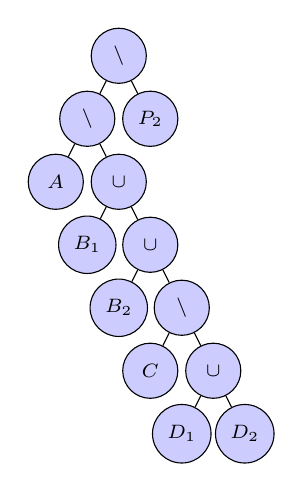
\begin{tikzpicture}[
mystyle/.style={draw, circle, minimum size = 0.7cm, fill = blue!20, font = \scriptsize},
sibling distance = 10mm,
level distance = 10mm,
scale = 0.8
]
\node[mystyle] {$\setminus$}
	child {node[mystyle] {$\setminus$}
		child {node[mystyle] {$A$}}
		child {node[mystyle] {$\cup$}
    	child {node[mystyle] {$B_1$}}
    	child {node[mystyle] {$\cup$}
    		child {node[mystyle] {$B_2$}}
    		child {node[mystyle] {$\setminus$}
    			child {node[mystyle] {$C$}}
    			child {node[mystyle] {$\cup$}
    				child {node[mystyle] {$D_1$}}
    				child {node[mystyle] {$D_2$}}
    			}
    		}
    	}
    }
	}
    child {node[mystyle] {$P_2$}};
\end{tikzpicture}

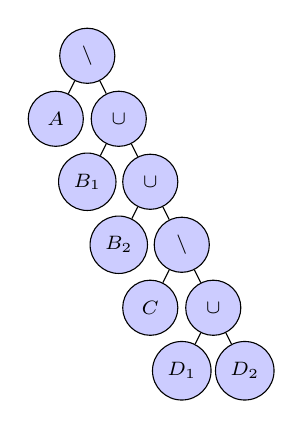
\begin{tikzpicture}[
mystyle/.style={draw, circle, minimum size = 0.7cm, fill = blue!20, font = \scriptsize},
sibling distance = 10mm,
level distance = 10mm,
scale = 0.8
]
\node[mystyle] {$\setminus$}
		child {node[mystyle] {$A$}}
		child {node[mystyle] {$\cup$}
    	child {node[mystyle] {$B_1$}}
    	child {node[mystyle] {$\cup$}
    		child {node[mystyle] {$B_2$}}
    		child {node[mystyle] {$\setminus$}
    			child {node[mystyle] {$C$}}
    			child {node[mystyle] {$\cup$}
    				child {node[mystyle] {$D_1$}}
    				child {node[mystyle] {$D_2$}}
    			}
    		}
    	}
    };
\end{tikzpicture}

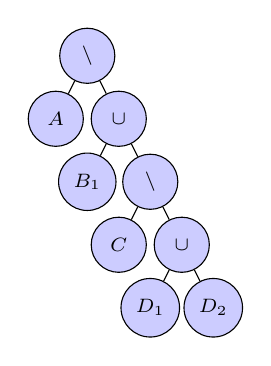
\begin{tikzpicture}[
mystyle/.style={draw, circle, minimum size = 0.7cm, fill = blue!20, font = \scriptsize},
sibling distance = 10mm,
level distance = 10mm,
scale = 0.8
]
\node[mystyle] {$\setminus$}
		child {node[mystyle] {$A$}}
		child {node[mystyle] {$\cup$}
    	child {node[mystyle] {$B_1$}}
    		child {node[mystyle] {$\setminus$}
    			child {node[mystyle] {$C$}}
    			child {node[mystyle] {$\cup$}
    				child {node[mystyle] {$D_1$}}
    				child {node[mystyle] {$D_2$}}
    			}
    		}
    };
\end{tikzpicture}

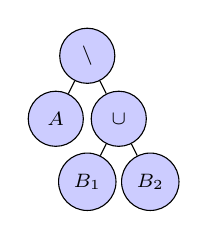
\begin{tikzpicture}[
mystyle/.style={draw, circle, minimum size = 0.7cm, fill = blue!20, font = \scriptsize},
sibling distance = 10mm,
level distance = 10mm,
scale = 0.8
]
\node[mystyle] {$\setminus$}
		child {node[mystyle] {$A$}}
		child {node[mystyle] {$\cup$}
    	child {node[mystyle] {$B_1$}}
    	child {node[mystyle] {$B_2$}
    	}
    };
\end{tikzpicture}

% \begin{tikzpicture}[
%   scale = 4,
%   decoration={
%       markings,
%       mark=at position 0.5 with {\arrow{>}}}
%   ]

% \coordinate (A) at (0,0.4);
% \coordinate (B) at (1,0.6);
% \fill[blue, fill opacity=0.5] (A)--(B)-|(1,1)--(0,1)--cycle;
% \fill[red, fill opacity=0.5] (A)--(B)-|(1,0)--(0,0)--cycle;
% \draw[green, very thick, postaction={decorate}] (A)--(B);
% \draw[very thick, black] (0,0) rectangle (1,1);
% \node at (0.5,0.75) {POSITIF};
% \node at (0.5,0.25) {NÉGATIF};

% \node[rotate=11.3099, below] at ($(A)!0.5!(B)$) {$ax+by+c=0$};

% \end{tikzpicture}

% \begin{tikzpicture}[
%   scale = 4,
%   decoration={
%       markings,
%       mark=at position 0.5 with {\arrow{>}}}
%   ]

% \coordinate (A) at (0.0596,0.7658);
% \coordinate (B) at (0.0050,0.3504);
% \coordinate (C) at (0.7742,0.2425);
% \coordinate (D) at (0.7384,0.8882);
% \coordinate (E) at (0.5832,0.6812);
% \coordinate (F) at (0.7530,0.2649);
% \coordinate (G) at (0.1272,0.2193);
% \coordinate (H) at (0.6590,0.3571);
% \coordinate (I) at (0.6575,0.9572);
% \coordinate (J) at (0.9776,0.4108);
% \coordinate (K) at (0.7784,0.6394);
% \coordinate (L) at (0.7474,0.9293);
% \coordinate (M) at (0.8673,0.3549);
% \coordinate (N) at (0.3368,0.0580);
% \coordinate (O) at (0.1714,0.3147);
% \coordinate (P) at (0.1176,0.5265);
% \coordinate (Q) at (0.7435,0.1821);
% \coordinate (R) at (0.1434,0.0814);
% \coordinate (S) at (0.4455,0.0079);
% \coordinate (T) at (0.8742,0.8670);

% \draw[very thick] (B)--(R)--(S)--(Q)--(J)--(T)--(L)--(I)--(A)--cycle;
% \fill[blue, fill opacity = 0.5] (B)--(R)--(S)--(Q)--(J)--(T)--(L)--(I)--(A)--cycle;
% \draw[black, very thick, postaction={decorate}] (B)--(R);
% \draw[black, very thick, postaction={decorate}] (R)--(S);
% \draw[black, very thick, postaction={decorate}] (S)--(Q);
% \draw[black, very thick, postaction={decorate}] (Q)--(J);
% \draw[black, very thick, postaction={decorate}] (J)--(T);
% \draw[black, very thick, postaction={decorate}] (T)--(L);
% \draw[black, very thick, postaction={decorate}] (L)--(I);
% \draw[black, very thick, postaction={decorate}] (I)--(A);
% \draw[black, very thick, postaction={decorate}] (A)--(B);

% \end{tikzpicture}

% \begin{tikzpicture}[
%   scale = 3,
%   decoration={
%       markings,
%       mark=at position 0.5 with {\arrow{>}}}
%   ]

% \coordinate (A) at (0,0.2);
% \coordinate (AA) at (0.4,0.6);
% \coordinate (B) at (1,0.2);
% \coordinate (C1) at (0.25,0.5);
% \coordinate (C2) at ($(C1)+(0.45,0)$);
% \coordinate (C3) at ($(C2)+(0,0.25)$);
% \coordinate (C4) at ($(C3)+(-0.45,0)$);
% \fill[blue, fill opacity=0.5] (A)--(AA)--(B)--(1,1)--(0,1)--cycle;
% \draw[fill=red!50!white] (C1)--(C2)--(C3)--(C4)--cycle;
% \draw[black, very thick, postaction={decorate}] (A)--(AA);
% \draw[black, very thick, postaction={decorate}] (AA)--(B);
% \draw[very thick] (0,0) rectangle (1,1);
% \foreach \pt in {C1,C2,C3,C4}{
% 	\draw[fill=red] (\pt) circle (0.3pt);
% }

% \end{tikzpicture}

% \begin{tikzpicture}[
%   scale = 4,
%   decoration={
%       markings,
%       mark=at position 0.5 with {\arrow{>}}}
%   ]

% \coordinate (C) at (0,0.8);
% \coordinate (D) at (1,0.2);

% \fill[red, fill opacity=0.5] (C)--(D)-|(1,1)--(0,1)--cycle;
% \draw[black, very thick, postaction={decorate}] (C)--(D);
% \draw[very thick] (0,0) rectangle (1,1);

% \node at (0.5,0.7) {\huge $H_2$};

% \end{tikzpicture}

% \begin{tikzpicture}[
%   scale = 4,
%   decoration={
%       markings,
%       mark=at position 0.5 with {\arrow{>}}}
%   ]

% \coordinate (A) at (0,0.4);
% \coordinate (B) at (1,0.6);
% \coordinate (C) at (0,0.8);
% \coordinate (D) at (1,0.2);
% \coordinate (I) at (0.5,0.5);

% % \fill[red!50!blue] (C)--(I)--(B)--(1,1)--(0,1)--cycle;

% \fill[blue!50!red, fill opacity=0.75] (C)--(I)--(B)--(1,1)--(0,1)--cycle;
% \fill[blue, fill opacity=0.25] (A)--(I)--(C)--cycle;
% \fill[red, fill opacity=0.25] (B)--(I)--(D)--cycle;
% \draw[black, very thick, dashed] (A)--(B);
% \draw[black, very thick, dashed] (C)--(D);
% \draw[black, very thick, postaction={decorate}] (C)--(I);
% \draw[black, very thick, postaction={decorate}] (I)--(B);
% \draw[very thick] (0,0) rectangle (1,1);

% \node at (0.5,0.8) {\huge $H_1 \cap H_2$};

% \end{tikzpicture}

% \begin{tikzpicture}[
%   scale = 4,
%   decoration={
%       markings,
%       mark=at position 0.5 with {\arrow{>}}}
%   ]

% \coordinate (A) at (0,0.4);
% \coordinate (B) at (1,0.6);
% \coordinate (C) at (0,0.8);
% \coordinate (D) at (1,0.2);
% \coordinate (I) at (0.5,0.5);

% % \fill[red!50!blue] (C)--(I)--(B)--(1,1)--(0,1)--cycle;

% \fill[blue!50!red, fill opacity=0.75] (A)--(I)--(D)--(1,1)--(0,1)--cycle;
% \draw[black, very thick, dashed] (A)--(B);
% \draw[black, very thick, dashed] (C)--(D);
% \draw[black, very thick, postaction={decorate}] (A)--(I);
% \draw[black, very thick, postaction={decorate}] (I)--(D);
% \draw[very thick] (0,0) rectangle (1,1);

% \node at (0.5,0.8) {\huge $H_1 \cup H_2$};

% \end{tikzpicture}

% \begin{tikzpicture}[
%   scale = 4,
%   decoration={
%       markings,
%       mark=at position 0.5 with {\arrow{>}}}
%   ]

% \coordinate (A) at (0,0.4);
% \coordinate (B) at (1,0.6);
% \coordinate (C) at (0,0.8);
% \coordinate (D) at (1,0.2);

% \fill[blue!50!red, fill opacity=0.75] (A)--(I)--(C)--cycle;
% \fill[blue, fill opacity=0.25] (C)--(I)--(B)--(1,1)--(0,1)--cycle;
% \fill[red, fill opacity=0.25] (A)--(I)--(D)--(1,0)--(0,0)--cycle;
% \draw[black, very thick, dashed] (A)--(B);
% \draw[black, very thick, dashed] (C)--(D);
% \draw[black, very thick, postaction={decorate}] (A)--(I);
% \draw[black, very thick, postaction={decorate}] (I)--(C);
% \draw[very thick] (0,0) rectangle (1,1);

% \end{tikzpicture}

% \tdplotsetmaincoords{60}{100}
%     \begin{tikzpicture}[tdplot_main_coords,scale=1,line join=round]
%     \pgfmathsetmacro\a{2}
%     \pgfmathsetmacro{\phi}{\a*(1+sqrt(5))/2}
%     \path 
%     coordinate(A) at (0,\phi,\a)
%     coordinate(B) at (0,\phi,-\a)
%     coordinate(C) at (0,-\phi,\a)
%     coordinate(D) at (0,-\phi,-\a)
%     coordinate(E) at (\a,0,\phi)
%     coordinate(F) at (\a,0,-\phi)
%     coordinate(G) at (-\a,0,\phi)
%     coordinate(H) at (-\a,0,-\phi)
%     coordinate(I) at (\phi,\a,0)
%     coordinate(J) at (\phi,-\a,0)
%     coordinate(K) at (-\phi,\a,0)
%     coordinate(L) at (-\phi,-\a,0); 
%     \draw[dashed, thick]    (B) -- (H) -- (F) 
%     (D) -- (L) -- (H) --cycle 
%     (K) -- (L) -- (H) --cycle
%     (K) -- (L) -- (G) --cycle
%     (C) -- (L) (B)--(K) (A)--(K)
%     ;
        
%         \draw[ultra thick]
%         (A) -- (I) -- (B) --cycle 
%         (F) -- (I) -- (B) --cycle 
%         (F) -- (I) -- (J) --cycle
%         (F) -- (D) -- (J) --cycle
%         (C) -- (D) -- (J) --cycle
%         (C) -- (E) -- (J) --cycle
%         (I) -- (E) -- (J) --cycle
%         (I) -- (E) -- (A) --cycle
%         (G) -- (E) -- (A) --cycle
%         (G) -- (E) -- (C) --cycle
%         ; 
%  \foreach \point/\position in {A/right,B/below,C/above,D/left,E/{above right},F/below,G/above,H/left,I/below,J/right,K/below,L/left}
% {
%     \fill (\point) circle (1.5pt);
%     \node[\position=3pt] at (\point) {$\point$};
% }

% \draw[fill=blue, fill opacity = 0.5] (3,3,5)--++(6,0,0)--++(0,-6,0)--++(-6,0,0)--cycle;

% \end{tikzpicture}

% \begin{tikzpicture}[font=\large]

% \coordinate[label=right:{$(v_{1_x},v_{1_y},v_{1_z})$}] (A) at (0,0);
% \coordinate[label=below right:{$(v_{2_x},v_{2_y},v_{2_z})$}] (B) at (1,2);
% \coordinate[label=above:{$(v_{3_x},v_{3_y},v_{3_z})$}] (C) at (-2,3);
% \coordinate (D) at (-0.25,1.5);
% \coordinate[label=above right:{$(n_{x},n_{y},n_{z})$}] (E) at ($(D)+1.25*(0.5,1)$);

% \draw[very thick, fill, color=blue, fill opacity = 0.5] (A)--(B)--(C)--cycle;
% \draw[very thick,->] (D)--(E);

% \foreach \pt in {A,B,C}{
% 	\draw[fill=black] (\pt) circle (1pt);
% }

% \end{tikzpicture}

% \begin{tikzpicture}[
% 	decoration={
%     	markings,
%     	mark=at position 0.5 with {\arrow{>}}}
% 	]

% \begin{scope}
% \fill[blue!50] (-4,4) -| (10,-4) -- cycle;
% \draw[black, very thick, postaction={decorate}]  (-4,4) -- (10,-4);
% \end{scope}

% \begin{scope}[xshift={15cm}]
% \fill[red!50] (-4,-1) -| (10,3) -- cycle;
% \draw[black, very thick, postaction={decorate}]  (-4,-1) -- (10,3);
% \end{scope}

% \end{tikzpicture}

% \begin{tikzpicture}[node distance = 2.5cm]

% \tikzstyle{startstop} = [rectangle, rounded corners, minimum width=3cm, minimum height=1cm,text centered, draw=black, fill=red!30]
% \tikzstyle{io} = [trapezium, trapezium left angle=70, trapezium right angle=110, minimum width=2cm, minimum height=1cm, text centered, draw=black, fill=blue!30, text width = 2cm]
% \tikzstyle{process} = [rectangle, minimum width=1.25cm, minimum height=1cm, text centered, draw=black, fill=orange!30]
% \tikzstyle{decision} = [diamond, minimum width=1.5cm, minimum height=0.5cm, text centered, draw=black, fill=green!30, text width = 1.25cm]
% \tikzstyle{arrow} = [thick,->,>=stealth]

% \node (in1) [io] {Entrée: Partie infraséculaire}; 
% \node (de1) [decision, below of =in1] {Pair ou Impair?};
% \node (pro1) [process, right of = de1, xshift = 1.5cm] {Additionner 11};
% \node (pro2) [process, below of = de1] {Diviser par 2};
% \node (de2) [decision, below of = pro2] {Pair ou Impair?};
% \node (pro3) [process, right of = de2, xshift = 1.5cm] {Additionner 11};
% \node (pro4) [process, below of = de2] {Modulo 7};
% \node (pro5) [process, below of = pro4, yshift = 0.75cm] {Soustraire de 7};
% \node (in2) [io, below of = pro5, yshift = 0.75cm] {Sortie: Décalage};

% \draw [arrow] (in1) -- (de1);
% \draw [arrow] (de1) -- (pro1) node[midway, above, lightgray] {impair};
% \draw [arrow] (de1) -- (pro2) node[midway, left, lightgray] {pair};
% \draw [arrow] (pro1) |- ($(de1)!0.6!(pro2)$);
% \draw [arrow] (pro2) -- (de2);
% \draw [arrow] (de2) -- (pro3) node[midway, above, lightgray] {impair};
% \draw [arrow] (de2) -- (pro4) node[midway, left, lightgray] {pair};
% \draw [arrow] (pro3) |- ($(de2)!0.6!(pro4)$);
% \draw [arrow] (pro4) -- (pro5);
% \draw [arrow] (pro5) -- (in2);

% \end{tikzpicture}

% \begin{tikzpicture}
% \begin{axis}[
% view={120}{30},
% xlabel={$x$},
% ylabel={$y$},
% zlabel={$z$},
% xmax=3,
% xmin=-3,
% ymax=3,
% ymin=-3,
% zmin=0,
% zmax=15,
% ticks=none,
% axis lines=center
% ]
% \addplot3 [surf,draw=none,restrict z to domain=0:9, data cs=polar, domain=0:360, y domain=0:3] (x, y, y^2);
% \end{axis}
% \end{tikzpicture}


% \begin{tikzpicture}

% % \tikzset{node style ge/.style={rectangle, minimum width=10mm, minimum height=4mm}}
% \tikzset{node style ge/.style={circle, minimum size=10mm}}
% % \tikzstyle{column 3}=[blue]
% % \tikzstyle{column 4}=[red]

% \matrix (A) [matrix of math nodes, row sep = 2mm] 
% { 
%   \text{Étape } 1: & 2^2 & 2 \times 2 \times 4 & 4^2 \\
%   \text{Étape } 2: & 4 & \textcolor{blue}{1}6 & 16 \\
%   \text{Étape } 3: & 5 & 6 & \textcolor{blue}{1}6 \\
%   \text{Étape } 4: & 5 & 7 & 6 \\
% };

% \node at ($(A-1-2)!0.65!(A-2-2)$) {\tiny{\textcolor{blue}{+1}}};
% \draw[blue,->]  (A-2-3.north west) to[bend right] ($(A-1-2)!0.7!(A-2-2.north east)$);

% \node at ($(A-2-3)!0.65!(A-3-3)$) {\tiny{\textcolor{blue}{+1}}};
% \draw[blue,->]  (A-3-4.north west) to[bend right] ($(A-2-3)!0.7!(A-3-3.north east)$);

% \end{tikzpicture}

% \tdplotsetmaincoords{60}{135}
% \begin{tikzpicture}[tdplot_main_coords]

% \def\hauteur{2}
% \def\rayon{1}
% \def\position{2}

% \draw[->] (0,0,0)--(2,0,0);
% \draw[->] (0,0,0)--(0,2,0);
% \draw[->] (0,0,0)--(0,0,6);

% \foreach \t in {-50,-40,...,120}{
%   \draw[blue, fill=blue, fill opacity=0.75]  
%     ({\rayon*cos(\t)},{\rayon*sin(\t)},{\position})--
%     ({\rayon*cos(\t+10)},{\rayon*sin(\t+10)},{\position})--++
%     (0,0,\hauteur)--
%     ({\rayon*cos(\t)},{\rayon*sin(\t)},{\position+\hauteur})--
%     cycle;
% }
% \draw[blue, fill=blue, fill opacity=0.5] (0,0,{\hauteur+\position}) circle (\rayon);

% \end{tikzpicture}

% \begin{tikzpicture}[scale=0.5]

% \coordinate[label=above left:{$(0,-2)$}] (A) at (0,-2);
% \coordinate[label=below right:{$(0,-4)$}] (B) at (0,-4);
% \coordinate[label=below right:{$(4,0)$}] (C) at (4,0);
% \coordinate[label=above left:{$(2,0)$}] (D) at (2,0);

% \fill[lightgray] (A)--(B)--(C)--(D)--cycle;

% \begin{scope}

% \clip (-1,-5) rectangle (5,1);
% \draw[domain = -1:5, blue, thick] plot (\x,{\x-2});
% \draw[domain = -1:5, blue, thick] plot (\x,{\x-4});

% \end{scope}

% \draw[->] (-1,0)--(6,0) node[below] {$x$};
% \draw[->] (0,-5)--(0,1) node[left] {$y$};

% \foreach \pt in {A,B,C,D}{
%   \draw[fill=black] (\pt) circle (2pt);
% }

% \end{tikzpicture}


% \begin{tikzpicture}

% \fill[green,fill opacity=0.5,even odd rule] (0,0) ellipse (3cm and 1cm) (0,0) circle (2cm);

% \fill[white] (0,0) circle (2cm);

% \draw[->] (-3.5,0)--(3.5,0) node[below] {$x$};
% \draw[->] (0,-2.5)--(0,2.5) node[left] {$y$};

% \draw[blue,thick] (0,0) circle (2cm);
% \draw[red,thick,dashed] (0,0) ellipse (3cm and 1cm);
% \draw[gray,thick,dashed] (0,0) ellipse (2.83cm and 0.94cm);

% \foreach \i in {-3,-2,-1,1,2,3}{
%   \draw (\i,0.1)--++(0,-0.2) node[below] {$\i$};
% }
% \foreach \j in {-2,-1,1,2}{
%   \draw (0.1,\j)--++(-0.2,0) node[left] {$\j$};
% }

% \end{tikzpicture}

% \opadd{3709}{4356}



% \begin{tikzpicture}[
%     row 1/.style={font=\textsl,font=\scriptsize,red!85, anchor=south, inner sep=1.5pt},
%     every node/.style={column sep=.25mm,row sep=0.5mm}]
%     \matrix (m) [matrix of math nodes,
%         nodes in empty cells,
%         %nodes=draw
%     ] 
%     {
%         & 1 & & 1 & \\
%         & 3 & 7 & 0 & 9 \\
%         & 4 & 3 & 5 & 6 \\
%         & 8 & 0 & 6 & 5 \\                       
%     };

%     \draw[-,color=black,semithick] (m-3-2.south west) -- (m-3-5.south east);
%     \node at ($(m-3-1.north east)!0.5!(m-2-1.north east)$) {+};
%     \draw[-,color=red,semithick] (m-2-4.south east)--(m-2-4.north west);
%     \draw[-,color=red,semithick] (m-2-5.south east)--(m-2-5.north west);

% \end{tikzpicture}



% \begin{tikzpicture}

% \draw[->] (-4,0)--(2.5,0) node[below] {$x$};
% \draw[->] (0,-2)--(0,2) node[left] {$y$};

% \draw[domain=0:2,thick,blue,samples=100] plot (\x,{sqrt(\x)});
% \draw[domain=0:2,thick,blue,samples=100] plot (\x,{-sqrt(\x)});

% \draw[fill=red,fill opacity=0.5] (-3,-0.05) rectangle (-1,0.05);
% \draw (-2,0.1)--(-2,-0.1) node[below] {$a$};
% \draw (-3,0.1)--(-3,-0.1) node[below] {$a-R$};
% \draw (-1,0.1)--(-1,-0.1) node[below] {$a+R$};

% \end{tikzpicture}

% \begin{tikzpicture}

% % Supporting structure
% \fill[pattern= north west lines,] (-2.5,2.41) rectangle (2.5,2.6);
% \draw(-2.5,2.41) -- (2.5,2.41);

% % Pulley
% \draw[fill = gray] (0,0) circle (1.5cm); % Big circle
% \draw[fill=lightgray] (0,0) circle (1.3cm); % Medium circle
% \draw[fill=white] (75:2.5) to[rounded corners=0.2cm] (0.2,-0.25) to[rounded corners=0.2cm] (-0.2,-0.25) -- (105:2.5) -- cycle;
% \draw[fill=darkgray] (0,0) circle (0.12cm); % Axle circle

% % Forces
% \draw[very thick] (-1.5,0)--++(0,-4);
% \draw[very thick] (1.5,0)--++(0,-6);

% \end{tikzpicture}

% \begin{tikzpicture}

% \draw (0,0) circle (6cm);
% \draw[fill=black] (0,0) circle (2pt);
% \draw (0,0) circle (3pt);
% \foreach \id in {1,2,...,12}{
%     \draw ($({90-30*\id}:6)$)--($({90-30*\id}:6.25)$);
%     \draw[fill=black] ($({90-30*\id}:4.5)$) circle (0.5pt);
%     \draw[fill=black] ($({90-30*\id}:4.25)$) circle (0.5pt);
%     \draw[fill=black] ($({90-30*\id}:7.5)$) circle (0.5pt);
%     \draw[fill=black] ($({90-30*\id}:7.75)$) circle (0.5pt);
% }
% \foreach \id in {1,2,...,60}{
%     \draw ($({90-6*\id}:6.15)$)--($({90-6*\id}:6.25)$);
% }
% \foreach \id in {1,2,...,12}{
%     \node at ($({90-30*\id}:5.5)$) {\large \id};
% }
% \foreach \id [evaluate={\lb=int(\id+12)}] in {1,2,...,12}{
%     \node at ($({90-30*\id}:6.5)$) {\large \lb};
% }
% \foreach \id [evaluate={\lb=int(\id+2*12)}] in {1,2,...,12}{
%     \node at ($({90-30*\id}:7)$) {\large \lb};
% }
% \foreach \id [evaluate={\lb=int(\id-12)}] in {1,2,...,12}{
%     \node at ($({90-30*\id}:5)$) {\large \lb};
% }

% \end{tikzpicture}

% \begin{tikzpicture}

% \boat{(0,0)}{225}{1}
% \boat{(0,8)}{-45}{1}

% \draw[very thick,->] (0,0)--++(225:2.5);
% \draw[very thick,->] (0,8)--++(-45:2.5);
% \draw[very thick] (0,0)--(0,8);

% \end{tikzpicture}

% \begin{tikzpicture}[
% scale=2,
% mydot/.style={
%   draw,
%   circle,
%   fill=black,
%   inner sep=1.5pt}
% ]
% \draw
%   (0,0) coordinate (A) --
%   (2,0) coordinate (B) --
%   ($ (A)!.5!(B) ! {sin(60)*2} ! 90:(B) $) coordinate (C) -- cycle;
% \coordinate (O) at
%   (barycentric cs:A=1,B=1,C=1);
% \draw (O) circle [radius=2*1.717/6];
% \draw (C) -- ($ (A)!.5!(B) $) coordinate (LC); 
% \draw (A) -- ($ (B)!.5!(C) $) coordinate (LA); 
% \draw (B) -- ($ (C)!.5!(A) $) coordinate (LB); 
% \foreach \Nodo in {A,B,C,O,LC,LA,LB}
%   \node[mydot] at (\Nodo) {};    
% \end{tikzpicture}

% \begin{tikzpicture}

% \foreach \i in {1,2,3,4,5,6}{
%   \node[above] at (\i,6.5) {\dice{\i}{red}{0.6}};
%   \node[left] at (0.5,7-\i) {\dice{\i}{blue}{0.6}};
%   \foreach[evaluate={\k=int(\i+\j)}] \j in {1,2,3,4,5,6}{
%       \node at (\i,7-\j) {\Large \k};
%   }
% }

% \end{tikzpicture}

% \begin{tikzpicture}[scale=0.25]

% \foreach \i in {1,2,...,5}{
% 	\node[above] at ($(\i,0)+(0.5,1)$) {\small\i};
% }

% \foreach \j [evaluate={\k=int(-1*\j+1)}] in {0,-1,...,-9}{
% 	\node[left,text=lightgray] at ($(1,\j)+(0,0.5)$) {\small\k};
% }

% \foreach \j in {0,-1,...,-9}{
% 	\foreach \i in {1,2,...,5}{
% 		\draw[thick] (\i,\j) rectangle++ (1,1);
% 	}
% }

% \foreach \i/\j/\k/\h in {
% 	1/2/3/0,
% 	1/2/4/-1,
% 	1/2/5/-2,
% 	1/3/4/-3,
% 	1/3/5/-4,
% 	1/4/5/-5,
% 	2/3/4/-6,
% 	2/3/5/-7,
% 	2/4/5/-8,
% 	3/4/5/-9
% }{
% 	\draw[thick,fill=red] (\i,\h) rectangle++ (1,1);
% 	\draw[thick,fill=red] (\j,\h) rectangle++ (1,1);
% 	\draw[thick,fill=red] (\k,\h) rectangle++ (1,1);
% }

% \begin{scope}[xshift=6cm]

% \foreach \j in {0,-1,...,-9}{
% 	\foreach \i in {1,2,3}{
% 		\draw[thick] (\i,\j) rectangle++ (1,1);
% 	}
% }

% \foreach \i/\j/\k/\h in {
% 	1/2/3/0,
% 	1/2/4/-1,
% 	1/2/5/-2,
% 	1/3/4/-3,
% 	1/3/5/-4,
% 	1/4/5/-5,
% 	2/3/4/-6,
% 	2/3/5/-7,
% 	2/4/5/-8,
% 	3/4/5/-9
% }{
% 	\node at ($(1,\h)+(0.5,0.5)$) {\small\i};
% 	\node at ($(2,\h)+(0.5,0.5)$) {\small\j};
% 	\node at ($(3,\h)+(0.5,0.5)$) {\small\k};
% }

% \end{scope}

% \end{tikzpicture}

% \begin{tikzpicture}

% \begin{scope}
% \edef\n{0}
% \foreach \idy in {1,2,...,10}{
% 	\pgfmathparse{\n-0.47}
% 	\xdef\n{\pgfmathresult}
% 	\foreach \idx in {1,2,...,5}{
% 		\node[rectangle,draw] (first) at (0,\n) {\phantom{5}};
% 		\node[rectangle,draw] (second) [right=0cm of first] {\phantom{5}};
% 		\node[rectangle,draw] (third) [right=0cm of second] {\phantom{5}};
% 		\node[rectangle,draw] (fourth) [right=0cm of third] {\phantom{5}};
% 		\node[rectangle,draw] (fifth) [right=0cm of fourth] {\phantom{5}};
% 	}
% }

% \end{scope}	

% \begin{scope}[xshift=3cm]
% \edef\n{0}

% \foreach \i/\j/\k in {
% 	1/2/3,
% 	1/2/4,
% 	1/2/5,
% 	1/3/4,
% 	1/3/5,
% 	1/4/5,
% 	2/3/4,
% 	2/3/5,
% 	2/4/5,
% 	3/4/5
% }{
% 	\pgfmathparse{\n-0.47}
% 	\xdef\n{\pgfmathresult}
% 	\node[rectangle,draw] (first) at (0,\n) {\i};
% 	\node[rectangle,draw] (second) [right=0cm of first] {\j};
% 	\node[rectangle,draw] (third) [right=0cm of second] {\k};
% }
% \end{scope}

% \end{tikzpicture}

% \begin{tikzpicture}[use Hobby shortcut]

% \draw (10:1) arc (10:80:1);
% \draw (10:4) arc (10:80:4);
% \draw[->] (-0.25,0)--(4.5,0);
% \draw[->] (0,-0.25)--(0,4.5);
% \draw[thick,fill=lightgray] (20:1)..(15:1.5)..(20:2)..(20:4) arc (20:70:4) ..(60:3)..(55:2)..(65:1.5)..(70:1) arc (70:20:1);
% \node[label=45:{$r=b$}] at (45:4) {};
% \node[label=45:{$r=a$}] at (45:1) {};
% \node[below right] at (20:2.5) {$\theta=\theta_1(r)$};
% \node[above left] at (55:2.5) {$\theta=\theta_2(r)$};

% \end{tikzpicture}



% \begin{tikzpicture}

% \def\Largeur{6}
% \def\Profondeur{3}
% \def\Hauteur{3}

% \begin{axis}[
%     hide axis,
%     view={120}{10},
%     axis lines=center,
%     xmin=-2,
%     xmax=7,
%     ymin=-2,
%     ymax=5,
%     zmin=-2,
%     zmax=5
% ]

% \coordinate (B1) at (0,0,0);
% \coordinate (B2) at (\Largeur,0,0) ;
% \coordinate (B3) at (\Largeur,\Profondeur,0);
% \coordinate (B4) at (0,\Profondeur,0);

% \coordinate (H1) at (0,0,\Hauteur);
% \coordinate (H2) at (\Largeur,0,\Hauteur) ;
% \coordinate (H3) at (\Largeur,\Profondeur,\Hauteur);
% \coordinate (H4) at (0,\Profondeur,\Hauteur);

% \fill[gray] (B1)--(B2)--(B3)--(B4)--cycle;
% \draw[fill=gray,fill opacity=0.5] (B4)--(B1)--(H1)--(H4)--cycle;
% \draw[fill=gray,fill opacity=0.5] (B1)--(B2)--(H2)--(H1)--cycle;
% \draw[fill=lightgray!25!white,fill opacity=0.5] (B2)--(B3)--(H3)--(H2)--cycle;
% \draw[fill=lightgray!25!white,fill opacity=0.5] (B3)--(B4)--(H4)--(H3)--cycle;

% \draw (B2)--(B3) node[midway,below] {$x$};
% \draw (B3)--(B4) node[midway,below] {$y$};
% \draw (B4)--(H4) node[midway,right] {$z$};

% \end{axis}

% \end{tikzpicture}

% \begin{tikzpicture}
% \node {$z$}
%     child {node {$x$} [sibling distance=1cm]
%       child {node {$u$}}
%       child {node {$v$}}
%     } 
%     child {node {$y$} [sibling distance=1cm]
%       child {node {$u$}}
%     }
%     child {node {$z$} [sibling distance=1cm]
%       child {node {$u$}}
%       child {node {$v$}}
%     }
%     ;
% \end{tikzpicture}

% \begin{tikzpicture}

% \draw[->] (-0.5,0)--(5,0) node[below] {$x$};
% \draw[->] (0,-0.5)--(0,5) node[left] {$y$};
% \draw[domain=1:4,thick,blue,samples=50] plot (\x,{sqrt(\x-1)+1});
% \draw[->,very thick] (2,{sqrt(2-1)+1})--++(2,{1/sqrt(2-1)}) node[right] {$\vec u$};
% \draw[->,very thick] (2,{sqrt(2-1)+1})--++(-1,{sqrt(2-1)/0.5}) node[left] {$\Delta f$};
% \draw (2,{sqrt(2-1)+1})--++(27:0.5) arc (27:117:0.5) node[midway, above] {$\theta$};
% \node[below] at (1,1) {$f(x,y)=k$};

% \end{tikzpicture}

% \begin{tikzpicture}
%   \begin{axis}[
%       view={110}{30},
%       xlabel={$x$},
%       ylabel={$y$},
%       zlabel={$z$},
%       axis equal,
%       axis lines=middle,
%       zmax=5,
%       ticks=none
%     ]
% \draw[red,thick] (0,0,0)--(1,0,0)--(1,4,0)--(0,4,0)--cycle;
% \draw[red,thick] (0,0,2)--(1,0,2)--(1,4,2)--(0,4,2)--cycle;
% \draw[red,thick,dashed] (0,0,0)--(0,0,2);
% \draw[red,thick] (1,0,0)--(1,0,2);
% \draw[red,thick] (1,4,0)--(1,4,2);
% \draw[red,thick] (0,4,0)--(0,4,2);
% \addplot3[surf,domain=0:90,y domain=0:90,fill opacity=0.25,blue!50!white,opacity=0.5] ({3*cos(x)*sin(y)},{6*sin(x)*sin(y)},{4*cos(y)});
% \node[above right] at (0,1,4) {$16x^2+4y^2+9z^2=144$};
% \end{axis}
% \end{tikzpicture}

% \begin{tikzpicture}
% \begin{axis}[
%     view={0}{90},
%     ticks=none,
%     xlabel={$x$},
%     ylabel={$y$},
% ]
% \addplot3[
% contour gnuplot={number=20,labels=false},
% domain=0.01:5,
% samples=100
% ] {exp(-y/x)};
% \addplot3[
% contour gnuplot={number=20,labels=false},
% domain=-5:-0.01,
% samples=100
% ] {exp(-y/x)};
% \end{axis}
% \end{tikzpicture}


% \begin{tikzpicture}

% \draw[->] (-3,0)--(3,0);
% \draw[->] (0,-3)--(0,3);

% \foreach \ang in {72,108,252,288}{
%   \draw[blue,thick] (0,0)--(\ang:2.75);
%   \node[blue] at (\ang:3) {0,2};
% }
% \foreach \ang in {54,126,234,304}{
%   \draw[red,thick] (0,0)--(\ang:2.75);
%   \node[red] at (\ang:3) {0,2};
% }
% \foreach \ang in {36,142,218,320}{
%   \draw[green,thick] (0,0)--(\ang:2.75);
%   \node[green] at (\ang:3) {0,2};
% }
% \foreach \ang in {18,158,200,338}{
%   \draw[black,thick] (0,0)--(\ang:2.75);
%   \node[black] at (\ang:3) {0,2};
% }

% \end{tikzpicture}


% \begin{tikzpicture}
%   \begin{axis}[
%     xlabel={$x$},              % default put x on x-axis
%     ylabel={$y$},  % default put y on y-axis
%     xtick={1},
%     ytick={1},
%     samples=100,
%     domain=0:2,
%     xmin=-0.25,xmax=2.75,
%     ymin=-0.25,ymax=2.5,
%     axis x line=middle,
%     axis y line=middle,
%   ]
%   \addplot[name path=func, black, thick, mark=none, ] {sqrt(x)} node[right] {$y=\sqrt{x}$};
%   \addplot[name path=line,thick] {x} node[right] {$y=x$};
%   \addplot fill between[
%     of = func and line,
%     soft clip={domain=0:1},
%     every even segment/.style  = {gray,opacity=.4}
%   ];
% \end{axis}
% \end{tikzpicture}

% \tdplotsetmaincoords{70}{110}%
% \tikzset{pics/3d bar/.style={code={%
%  \tikzset{3d bar/.cd,#1}
%  \path[3d bar/x face] (\mydx/2,\mydy/2,0) -- (\mydx/2,\mydy/2,\myh)
%     -- (-\mydx/2,\mydy/2,\myh) -- (-\mydx/2,\mydy/2,0) -- cycle;
%  \path[3d bar/y face] (\mydx/2,\mydy/2,0) -- (\mydx/2,\mydy/2,\myh)
%     -- (\mydx/2,-\mydy/2,\myh) -- (\mydx/2,-\mydy/2,0) -- cycle;
%  \path[3d bar/z face] (\mydx/2,\mydy/2,\myh) -- (-\mydx/2,\mydy/2,\myh)
%     -- (-\mydx/2,-\mydy/2,\myh) -- (\mydx/2,-\mydy/2,\myh) -- cycle;
%     }},3d bar/.cd,dx/.store in=\mydx,dx=1,dy/.store in=\mydy,dy=1,
%         h/.store in=\myh,h=1,x face/.style={draw=blue!50,fill=cyan!20},
%         y face/.style={draw=blue!50,fill=cyan!50},
%         z face/.style={draw=blue!50,fill=cyan!30}}

% \begin{tikzpicture}[tdplot_main_coords]
%  \begin{scope}[declare function={f(\x,\y)=1+3*exp(-(\x)/5-(\y)/4);% function
%     n=5;% steps
%     xmin=0;xmax=5;ymin=0;ymax=5;}]
%   \pgfmathtruncatemacro{\myn}{n}
%   \tikzset{3d bar/dx/.evaluated={(xmax-xmin)/n},
%      3d bar/dy/.evaluated={(ymax-ymin)/n}}
%   \foreach \i in {1,...,\myn}
%    {\foreach \j in {1,...,\myn}
%    {\pgfmathsetmacro{\myx}{xmin+(\i-0.5)*(xmax-xmin)/\myn}
%     \pgfmathsetmacro{\myy}{ymin+(\j-0.5)*(ymax-ymin)/\myn}
%     \pgfmathsetmacro{\myf}{f(\myx,\myy)}
%     \path (\myx,\myy,0) pic{3d bar={h=\myf}};}}  
%  \end{scope}
%  %
%  \begin{scope}[xshift=7cm,
%      declare function={f(\x,\y)=0.5+3*exp(-\x/5-\y/4);% function
%      n=20;% steps
%      xmin=0;xmax=5;ymin=0;ymax=5;}]
%   \pgfmathtruncatemacro{\myn}{n}
%   \tikzset{3d bar/dx/.evaluated={(xmax-xmin)/n},
%      3d bar/dy/.evaluated={(ymax-ymin)/n}}
%   \foreach \i in {1,...,\myn}
%    {\foreach \j in {1,...,\myn}
%    {\pgfmathsetmacro{\myx}{xmin+(\i-0.5)*(xmax-xmin)/\myn}
%     \pgfmathsetmacro{\myy}{ymin+(\j-0.5)*(ymax-ymin)/\myn}
%     \pgfmathsetmacro{\myf}{f(\myx,\myy)}
%     \path (\myx,\myy,0) pic{3d bar={h=\myf}};}}  
%  \end{scope}
% \end{tikzpicture}


% \begin{tikzpicture}

% \begin{axis}[
%   samples=200,
%   xmin=0,
%   xmax=6,
%   ymin=-1.2,
%   ymax=1.2,
%   axis x line=middle,
%   axis y line=middle,
%   xlabel={$x$},
%   ylabel={$y$},
%   minor tick num=0,
%   xtick distance=10,
%   ytick distance=1,
%   x label style={at={(axis description cs:1,0.5)},anchor=north},
%   y label style={at={(axis description cs:0,1)},anchor=east}
% ]

% \addplot[thick,color=blue,domain=0:5.9]{exp(-x)*sin(deg(3*x))};
% \addplot[thick,color=red,dotted,domain=0:5.9]{exp(-x)};
% \addplot[thick,color=red,dotted,domain=0:5.9]{-exp(-x)};

% \end{axis}

% \end{tikzpicture}


% \begin{tikzpicture}

% \draw[thick] (-4,0)--(-2,0) node[below] {$a-R$};
% \draw[thick,->] (2,0)--(4,0) node[below,pos=0] {$a+R$};
% \draw[red,very thick] (-2,0)--(2,0) node[below,pos=0.5,text=black] {$a$};

% \draw [decorate, decoration = {brace}] (-2,0.2) --  (2,0.2) node[above,pos=0.5] {Intervalle de convergence pour $\abs{x-a}<R$};
% \draw [decorate, decoration = {brace, mirror}] (-4,-0.5) --  (-2,-0.5);
% \draw [decorate, decoration = {brace, mirror}] (2,-0.5) --  (4,-0.5);

% \draw[<->] (-3,-0.7)--++(0,-0.2)--++(6,0)--++(0,0.2);
% \node at (0,-1.2) {Intervalle de divergence pour $\abs{x-a}>R$};

% \draw[fill=white] (-2,0) circle (2pt);
% \draw[fill=white] (2,0) circle (2pt);
% \draw[fill=red,red] (0,0) circle (2pt);


% \end{tikzpicture}

% \begin{tikzpicture}

% \begin{axis}[
%   samples=100,
%   domain=-4:4,
%   xmin=-4,
%   xmax=4,
%   ymin=-1.5,
%   ymax=1.5,
%   axis x line=middle,
%   axis y line=middle,
%   xlabel={$x$},
%   ylabel={$y$},
%   marks=none,
%   minor tick num=0,
%   x label style={at={(axis description cs:1,0.5)},anchor=south},
%   y label style={at={(axis description cs:0.5,1)},anchor=east}
% ]

% \addplot[color=black]{sin(deg(x))};

% \end{axis}

% \end{tikzpicture}

% \begin{tikzpicture}[domain=-3:3,samples=100]

% \draw[black] plot (\x,1);
% \draw[blue] plot (\x,{1-(\x)^2/4});
% \draw[red] plot (\x,{1-(\x)^2/4+(\x)^4/64});
% \draw[green] plot (\x,{1-(\x)^2/4+(\x)^4/64-(\x)^6/2304});
% \draw[orange] plot (\x,{1-(\x)^2/4+(\x)^4/64-(\x)^6/2304+(\x)^8/147456});

% \end{tikzpicture}

% \begin{tikzpicture}
%     \begin{axis}[width=\textwidth, height=0.5*\textwidth, xlabel=$x$]
%     \addplot+[id=parable,domain=0:20, samples=500, mark=none, width=2pt]
%     gnuplot{besj0(x)} node[pin=95:{$J_0(x)$}]{};
%     \addplot+[id=parable,domain=0:20, samples=500, mark=none, width=2pt, color=red]
%     gnuplot{besj1(x)} node[pin=130:{$J_1(x)$}]{};
%     \addplot+[id=parable2,domain=0:20, samples=500, mark=none, width=2pt, color=black]
%     gnuplot{2*1/x*besj1(x)-besj0(x)} node[pin=-140:{$J_2(x)$}]{};
%    \end{axis}
% \end{tikzpicture}

% \begin{tikzpicture}

% \tkzInit[xmin=-3,xmax=9,ymin=-2,ymax=8]
% \tkzGrid[sub,color=gray!50!white]
% \tkzDrawXY
% \tkzClip

% \tkzDefPoint[label={left:$S\left(x_S;y_S\right)$}](-1,5){S} 
% \tkzDefShiftPoint[S](1,0){horizontale}
% \tkzDefPoint[label={right:$A\left(x_A;y_A\right)$}](5,7){A} 
% \tkzDefPoint[label={right:$B\left(x_B;y_B\right)$}](7,-1){B}

% \tkzDrawLine[dashed,add=0 and 20,very thick](S,horizontale)
% \tkzDrawSegments[very thick](S,A S,B)

% \tkzFillAngle[size=3cm,fill=blue,fill opacity=0.5](horizontale,S,A)
% \tkzMarkAngle[size=3cm,blue,very thick](horizontale,S,A)
% \tkzLabelAngle[pos=3,right,text=blue](horizontale,S,A){$\theta_{SA}$}

% \tkzFillAngle[size=2cm,fill=red,fill opacity=0.5](B,S,horizontale)
% \tkzMarkAngle[size=2cm,red,very thick](B,S,horizontale)
% \tkzLabelAngle[pos=2,right,text=red](B,S,horizontale){$\theta_{SB}$}

% \tkzDefLine[bisector](B,S,A) \tkzGetPoint{bissectrice}
% \tkzDrawLine[add=0 and 20,green,very thick](S,bissectrice)
% \tkzLabelLine[green,pos=0.5,sloped,below](S,bissectrice){Bissectrice}
% \tkzFillAngle[size=4cm,fill=green,fill opacity=0.5](bissectrice,S,horizontale)
% \tkzMarkAngle[size=4cm,green,very thick](bissectrice,S,horizontale)
% \tkzLabelAngle[pos=4,text=green,right](bissectrice,S,horizontale){$\theta_{\text{bissectrice}}=\tfrac{1}{2}\left(\theta_{SA}+\theta_{SB}\right)$}

% \tkzDrawPoints(A,B,S)

% \end{tikzpicture}

% \tdplotsetmaincoords{75}{22}
% \begin{tikzpicture}[tdplot_main_coords,scale=5,font=\Large]

% \coordinate (A) at (0,0,0); 
% \coordinate (B) at ($(A)+(1.2,0,0)$); 
% \coordinate (C) at ($(B)+(0,1.2,0)$);
% \coordinate (D) at ($(C)+(-1.2,0,0)$);

% \coordinate (A1) at ($(A)+(0,0,2)$);
% \coordinate (B1) at ($(B)+(0,0,2)$);
% \coordinate (C1) at ($(C)+(0,0,2)$);
% \coordinate (D1) at ($(D)+(0,0,2)$);

% \coordinate (S1) at ($(A1)+(-0.1,-0.1,0)$);
% \coordinate (S2) at ($(B1)+(0.1,-0.1,0)$);
% \coordinate (S3) at ($(C1)+(0.1,0.1,0)$);
% \coordinate (S4) at ($(D1)+(-0.1,0.1,0)$);

% \coordinate (F) at (0.6,0.6,2.7);

% \draw[thick] (A)--(B) node[midway,below] {12}--(C) node[midway,below right] {12};
% \draw[dashed,thick] (C)--(D)--(A);
% \draw[dashed,thick] (A1)--(B1)--(C1)--(D1)--cycle;
% \draw[thick] (A)--(A1);
% \draw[thick] (B)--(B1) node[midway,right] {20};
% \draw[thick] (C)--(C1);
% \draw[thick,dashed] (D)--(D1);

% \draw[ultra thick] (S1)--(S2) node[midway,below] {14}--(S3) node[midway,below right] {14}--(S4)--cycle;
% \draw[ultra thick] (S1)--(F);
% \draw[ultra thick] (S2)--(F);
% \draw[ultra thick] (S3)--(F);
% \draw[ultra thick,dashed] (S4)--(F);

% \end{tikzpicture}


% \tdplotsetmaincoords{70}{110}
% \begin{tikzpicture}[tdplot_main_coords]

% \draw[thick,->] (-4,0,0)--(4,0,0) node[below left] {$x$};
% \draw[thick,->] (0,-4,0)--(0,4,0) node[right] {$y$};
% \draw[thick,->] (0,0,-0.25)--(0,0,5) node[left] {$z$};

% \tdplotdrawarc{(0,0,0)}{3}{0}{360}{anchor=north}{}
% \tdplotdrawarc{(0,0,4)}{1}{0}{360}{anchor=north}{}

% \end{tikzpicture}

% \begin{tikzpicture}

% \begin{axis}[
%   view={110}{30},
%   colormap/blackwhite,
%   ticks=none,
%   xlabel={$x$},
%   ylabel={$y$},
%   zlabel={$z$}
% ]

% \addplot3[surf,domain=0:1,y domain=0:360,z buffer=sort]({x*cos(y)},{x*sin(y)},{x});
% \addplot3[surf,domain=0:360,y domain=0:45,z buffer=sort]({1.4142*cos(x)*sin(y)},{1.4142*sin(x)*sin(y)},{1.4142*cos(y)});

% \end{axis}

% \end{tikzpicture}

% \tdplotsetmaincoords{70}{110}
% \begin{tikzpicture}[tdplot_main_coords]

% \draw[thick,->] (-1,0,0)--(5,0,0) node[below left] {$x$};
% \draw[thick,->] (0,-1,0)--(0,5,0) node[right] {$y$};
% \draw[thick,->] (0,0,-0.25)--(0,0,4) node[left] {$z$};

% \draw[fill=black] (2,2,0) circle (2pt) node[right] {$(x,y,0)$};
% \draw[fill=black] (2,2,3) circle (2pt) node[right] {$P=(\rho,\theta,\phi)$};
% \draw[dashed] (0,0,0)--(2,2,0) node[midway,right=2pt] {$r$}--(2,2,3);
% \draw (1,0,0) arc (0:45:1) node[midway,below] {$\theta$};
% \draw[very thick] (0,0,0)--(2,2,3);

% \tdplotsetthetaplanecoords{60}
% \tdplotdrawarc[tdplot_rotated_coords]{(0,0,0)}{1}{0}%
% {35}{anchor=south}{$\phi$}

% \end{tikzpicture}

% \begin{tikzpicture}[use Hobby shortcut]

% \draw[->,thick] (0,0)--(4,0) node[below] {$u$};
% \draw[->,thick] (0,0)--(0,4) node[left] {$v$};
% \draw[fill=lightgray] (1,1)..(2,0.75)..(3,1.5)..(3.5,3)..(2,3.5)..(1,1);
% \node[right] at (3.5,2) {$D'$};
% \draw[->,thick] (3,3.75) to [out=45,in=135] (6,3.75);
% \node[above] at (4.5,4.5) {$\mathscr{T}$};
% \draw[fill=black] (2.5,2) circle (1pt);
% \draw[dashed] (2.5,2)--(0.7,-3.25);
% \draw[dashed] (2.5,2)--(3.3,-3.25);

% \begin{scope}[xshift=5cm]
% \draw[->,thick] (0,0)--(4,0) node[below] {$x$};
% \draw[->,thick] (0,0)--(0,4) node[left] {$y$};
% \draw[fill=lightgray] (1,1.1)..(2,0.8)..(3,1.1)..(3.5,2.75)..(2,3.25)..(1.5,3.4)..(1,1.1);
% \node[right] at (3.6,2) {$D$};
% \draw[fill=black] (2.5,2) circle (1pt);
% \draw[dashed] (2.5,2)--(0.7,-3.25);
% \draw[dashed] (2.5,2)--(3.3,-3.25);
% \end{scope}

% \begin{scope}[yshift=-6cm]
% \draw[thick] (0,0)--(4,0);
% \draw[thick] (0,0)--(0,4);
% \draw (2,2) circle (1.5cm);
% \node[label=below left:{$P'$}] (A) at (1.3,1.5) {};
% \node[label=right:{$Q'$}] (B) at (2.3,1.5) {};
% \node (C) at (2.3,2.5) {};
% \node[label=above:{$R'$}] (D) at (1.3,2.5) {};
% \draw[fill=lightgray] (1.3,1.5)--(2.3,1.5)--(2.3,2.5)--(1.3,2.5)--cycle;
% \foreach \pt in {A,B,C,D} {\draw[fill=black] (\pt) circle (1pt);}
% \draw[dotted] (1.3,0) node[below] {$u$} -- (1.3,1.5);
% \draw[dotted] (2.3,0) node[below] {$u+\Delta u$} -- (2.3,1.5);
% \draw[dotted] (0,1.5) node[left] {$v$} -- (1.3,1.5);
% \draw[dotted] (0,2.5) node[left] {$v+\Delta v$} -- (1.3,2.5);
% \draw[->,thick] (3,3.75) to [out=45,in=135] (6,3.75);
% \node[above] at (4.5,4.5) {$\mathscr{T}$};
% \end{scope}

% \begin{scope}[yshift=-6cm,xshift=5cm]
% \draw[thick] (0,0)--(4,0);
% \draw[thick] (0,0)--(0,4);
% \draw (2,2) circle (1.5cm);
% \node (A) at (1.25,1) {};
% \node (B) at (3,1.25) {};
% \node (C) at (2.75,3) {};
% \node (D) at (0.75,2.8) {};
% \draw[fill=lightgray] (1.25,1)..(2,1.15)..(3,1.25)..(2.5,2)..(2.75,3)..(2,2.9)..(0.75,2.8)--(1.25,1);
% \foreach \pt in {A,B,C,D} {\draw[fill=black] (\pt) circle (1pt);}
% \node[below left] at (A) {$P$};
% \node[above right] at (B) {$Q$};
% \node[above left] at (D) {$R$};
% \end{scope}

% \end{tikzpicture}

% \begin{tikzpicture}[scale=2]

% \draw[->] (-0.5,0)--(2.5,0) node[below] {$x$};
% \draw[->] (0,-2.5)--(0,0.5) node[left] {$y$};

% \foreach \i in {1,2}{
%   \draw (\i,-0.1)--++(0,0.2) node[above] {\i};
%   \draw (-0.1,-\i) node[left] {-\i} --++(0.2,0);
% }

% \draw[thick,fill=lightgray] (1,0)--(2,0) node[midway,above] {$L_1$} --(0,-2) node[midway,below right] {$L_2$} -- (0,-1) node[midway,left] {$L_3$} --cycle node[above left,midway] {$L_4$};

% \draw[->,line width=2pt] (2,-1)--++(2,0);

% \begin{scope}[xshift=6cm,yshift=-2cm]

% \draw[thick,fill=lightgray] (1,1)--(2,2) node[midway,right] {$L_1'$} --(-2,2) node[midway,above right] {$L_2'$} -- (-1,1) node[midway,left] {$L_3'$} --cycle node[below right,midway] {$L_4'$};

% \draw[->] (-2.5,0)--(2.5,0) node[below] {$u$};
% \draw[->] (0,-0.5)--(0,2.5) node[left] {$v$};

% \foreach \i in {1,2}{
%   \draw (\i,-0.1) node[below] {\i}--++(0,0.2);
%   \draw (-\i,-0.1) node[below] {-\i} --++(0,0.2);
%   \draw (-0.1,\i) node[left] {\i} --++(0.2,0);
% }

% \end{scope}

% \end{tikzpicture}

% \begin{tikzpicture}
% \draw[->] (-2,0)--(5,0) node[below]{$x$};
% \draw[->] (0,-2)--(0,5) node[left]{$y$};
% \draw[thick,blue,domain=-2:1.61] plot (\x,{exp(\x)});
% \draw[thick,blue,domain=0.1353:5,samples=50] plot (\x,{ln(\x)});
% \draw[thick,domain=-2:5] plot (\x,{\x});
% \foreach \i in {1} {
%   \draw (\i,-0.1) node[below] {$\i$}--++(0,0.2);
%   \draw (-0.1,\i) node[left] {$\i$}--++(0.2,0);
% }
% \node[above left] at (0,0) {$0$};
% \node[right] at (1.4,4) {$y=e^x$};
% \node[below right] at (3,1.09) {$y=\ln(x)$};
% \node[below right] at (3,3) {$y=x$};
% \node[right] at (-2.5,-2.5) {$\lim\limits_{x\to -\infty} e^x=0$};
% \node[right] at (-2.5,-3.5) {$\lim\limits_{x\to 0^{+}} \ln(x)=-\infty$};
% \node[right] at (2.5,-2.5) {$\lim\limits_{x\to \infty} e^x=\infty$};
% \node[right] at (2.5,-3.5) {$\lim\limits_{x\to 0^{-}} \ln(x)=\infty$};
% \end{tikzpicture}

% \begin{tikzpicture}
% \draw[->] (-5,0)--(5,0) node[below]{$x$};
% \draw[->] (0,-4)--(0,4) node[left]{$y$};
% \draw[thick,black,domain=-2.1:2.1,samples=50] plot(\x,{sinh(\x)});
% \draw[thick,blue,domain=-2:2,samples=50] plot(\x,{cosh(\x)});
% \draw[thick,blue,domain=-5:5,samples=50] plot(\x,{tanh(\x)});
% \node[above] at (4,1) {$y=\tanh(x)$};
% \node[left] at (-2,-3.5) {$y=\sinh(x)$};
% \node[left] at (-2,3.5) {$y=\cosh(x)$};
% \end{tikzpicture}

\end{document}